\chapter{Measuring intensities}
An image contains one type of information: the intensities of the pixels in the image. In this chapter, we will show you how to work with this intensity information in a quantitative way. We will look at intensity distributions and how to perform measurements based on the intensity distributions in regions of the image (e.g. a cell). 

\section{Histograms}
Each pixel in an image has an intensity (a pixel value). The intensity histogram of an image is a plot that shows the distribution of pixel counts over a range of intensity values, typically the bit-depth of the image or the range between the minimum and maximum values within the image. The histogram can be used to examine the signal and background levels (useful when you want to identify objects of interest).

\begin{taskbox}{Working with histograms}
\begin{enumerate}
	\item Open the image hela-cells.tif in /mod2/data. This is another standard Fiji sample image showing HeLa cells. Lysosomes are red, mitochondria green and the nucleus blue. 
	\item We can show the histogram with \texttt{[Analyze > Histogram]}. The histogram is displayed in a new window (Fig. \ref{fig:histogram}). The x-axis shows the pixel value and the y-axis the count. Note that the histogram refers to the channel that was active when the command was called.
	
	\begin{minipage}[t]{\linewidth}
		\begin{center}
		\adjustbox{valign=t}{%
			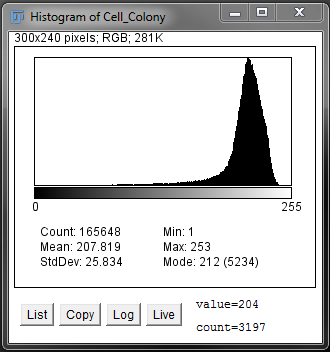
\includegraphics[width=0.4\textwidth]{mod2/figures/histogram.png}%
		}
		\medskip
		\captionof{figure}{Histogram.}\label{fig:histogram}
		\end{center}
	\end{minipage}
	
	\item Obtain the highest and lowest intensities from the histogram. What does the histogram range tell you?
	\item Click on [list] to obtain a list with values and counts. [Log] displays the same histogram on a log-scale.
	\item Click on [live] in the histogram dialog and change the channel. Observe the changes in the histogram and note the color changes in the depicted colormap bar.
	
\end{enumerate}

\end{taskbox}

\section{ROIs and the ROI Manager}
We now introduce a very powerful concept that is widely used for many types of analyses - the region of interest. Many operations can be applied to parts of the image when a region is selected by \emph{ROI} (region-of-interest) tools. The shape of the ROI is arbitrary; it can consist of a geometric shape, such as a circle or a line, but can be any selection of pixels. You already used ROIs when you selected a line or a point! Next, we will cover some basic ROI operations.

\begin{taskbox}{Working with ROIs}

One of the operations you can perform on a ROI is cropping:
\begin{enumerate}
	\item Open any image. Duplicate the image. Select a region by a rectangular ROI. Then, perform \texttt{[Image > Crop]} on the duplicate. Close the cropped image.
	\item Duplicate the original image again. Use the freehand selection to create a ROI on the duplicate. Crop the image. Note that the minimum and maximum values of your ROI have been used to determine a rectangular selection for the cropping.
\end{enumerate}

ROIs can be used to create image masks. An image masks is a binary image that define which parts of the image to analyze or measure.

\begin{enumerate}
	\item Open any image. Duplicate the image. Create a few circular ROIs (press <shift> during creation to keep multiple ROIs). 
	\item Use \texttt{[Edit > Clear Outside]} and then \texttt{[Edit > Fill]} to generate a mask image (this should look similar to fig. \ref{fig:binary-mask}. The 'Clear' command fills the respective area with the background color, 'fill' with the foreground color.
	
	\begin{minipage}[t]{\linewidth}
		\begin{center}
		\adjustbox{valign=t}{%
			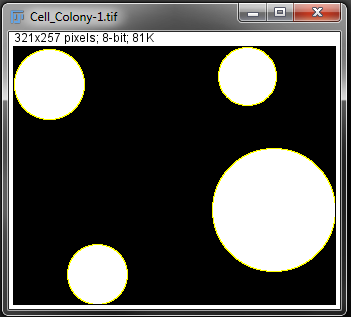
\includegraphics[width=0.4\textwidth]{mod2/figures/binary-mask.png}%
		}
		\medskip
		\captionof{figure}{Example binary mask.}\label{fig:binary-mask}
		\end{center}
	\end{minipage}
	
	\item Undo what you have done with \texttt{[Edit > Undo]}. You will notice that, in contrast to other programs, Fiji only allows to undo the most recent operation. This is done to minimize memory consumption. \texttt{[File > Revert]} allows you to go back to the last saved state.
	\item Go back to the original image. Use the command \texttt{[Edit > Selection > Create Mask]} to directly generate a mask image.
\end{enumerate}

Operations are usually performed on the selected ROIs and on the whole image if no selections exist. 
\begin{enumerate}
	\item Open any image. Duplicate the image. Select any ROI you like. 
	\item Observe that \texttt{[Edit > Invert]} only affects the selected pixels. Undo the inversion.
\end{enumerate}

Finally, there are several operations that work on a ROI itself without changing pixel values \texttt{[Edit > Selection > ...]}, see fig. \ref{fig:selection-options}. Let us explore a few of those options.

\begin{minipage}[t]{\linewidth}
		\begin{center}
		\adjustbox{valign=t}{%
			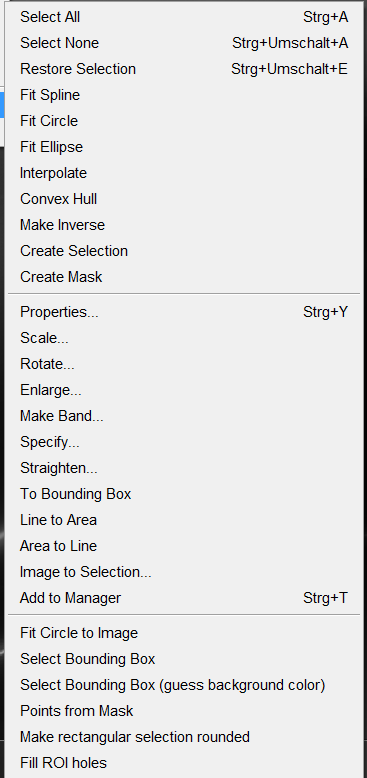
\includegraphics[width=0.4\textwidth]{mod2/figures/selection-options.png}%
		}
		\medskip
		\captionof{figure}{Selection options.}\label{fig:selection-options}
		\end{center}
	\end{minipage}


\begin{enumerate}
	\item Open an image, duplicate and draw a freehand selection with an outline that includes inner parts that are not selected. Fit a spline \texttt{[Fit Spline]}. This creates a smoothed version of the selection where individual points can now be dragged around and the shape can be changed. This can be useful to correct the outline of a shape (e.g. a worm or a cell). 
	\item Use \texttt{[To Bounding Box]}. This creates a rectangular region that just fits over the selection (this is the same as the crop area). Undo the last operation.
	\item Use \texttt{[Convex Hull]}. This creates an outline of the selection, where a straight line between every pair of points within the ROI is also within the ROI (Definition of a convex object in Euclidean space). This can be useful if you want to measure the extent of an object with an irregular shape. Undo the last operation.
	\item Explore the operations \texttt{[Scale]}, \texttt{[Make Inverse]}, \texttt{[Enlarge]} and \texttt{[Rotate]}.
	\item Each ROI has properties that can be displayed and changed with \texttt{[Properties]}. Especially useful when you work with multiple ROIs (and the ROI Manager, see below), can be ROI names (Fig. \ref{fig:roi-properties}). If you need the ROI coordinates outside Fiji, you can list the coordinates of the ROI as well.
	
	\begin{minipage}[t]{\linewidth}
		\begin{center}
		\adjustbox{valign=t}{%
			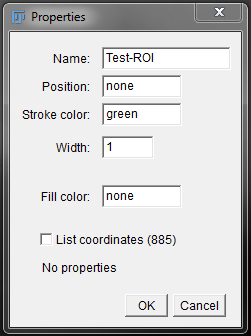
\includegraphics[width=0.4\textwidth]{mod2/figures/roi-properties.png}%
		}
		\medskip
		\captionof{figure}{ROI properties.}\label{fig:roi-properties}
		\end{center}
	\end{minipage}
	
\end{enumerate}

\end{taskbox}

\minisec{Managing multiple ROIs}
Fiji has an ROI manager to assist when you work with multiple ROIs. Open the ROI manager with \texttt{[Analyze > Tools > ROI Manager...]}. The manager allows you to add, delete and modify existing ROIs, save and load ROI coordinates, and change their display properties (Fig. \ref{fig:roi-manager}).

\begin{figure}[!ht]
	\begin{center}
		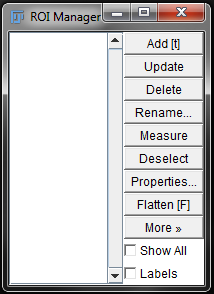
\includegraphics[width=0.3\textwidth]{mod2/figures/roi-manager.png}
		\caption{ROI manager.}\label{fig:roi-manager}
	\end{center}
\end{figure}

\begin{taskbox}{Working with the ROI Manager}
\begin{enumerate}
	\item Open the image hela-cells.tif in /mod2/data.
	\item Open the ROI Manager with \texttt{[Analyze > Tools > ROI Manager...]}.
	\item For the following analysis, we will only work on the bottom-most cell. Select the blue channel showing the nucleus. Use the ROI tools to create an accurate outline of the nucleus and add the selected region to the ROI manager. Rename the ROI to 'Nucleus'.
	\item Select the blue channel showing the mitochondria. In this channel, we can estimate the cell outline - create the outline and add the selected region to the ROI manager, rename ROI to 'Cell'.
	\item Let's say the task we want to solve is get the area of the cell, excluding the nucleus, for our further analysis. We now explore an option using the ROI manager, we will later explore another way using masks and image math. Select 'Nucleus' and 'Cell ROIs simultaneously. Then go to the [More>>] button and select the XOR operation. 
\emph{XOR} is the \emph{exclusive or} (exclusive disjunction). This is a logical operation that we apply to the ROIs. The XOR function returns the area where both inputs differ, i.e. not overlap. As the 'nucleus' ROI is located within the 'Cell' ROI, this subtracts the nucleus from the cell. Add the resulting ROI to the ROI Manager and rename to 'Cytoplasm'.
	\item Select all ROIs and save them on disk - we will use these ROIs for measurements. 
\end{enumerate}

\end{taskbox}

\section{Measurements}

The easiest way to read pixel values is moving the mouse pointer over individual pixels and reading their intensity value in the main Fiji bar. The histogram allows us to get the distribution of pixel intensities. Fiji has the function \texttt{[Analyze > Measure]} to obtain statistical information about pixel values within a ROI. \texttt{[Analyze > Set Measurements...] }allows us to select the parameters we want to measure. For example, following parameters can be obtained (Fig. \ref{fig:set_measurements-dialog}):
\begin{description}
	\item[Area] Area of selection in square pixels. If the image is calibrated, Area is displayed in according units.
	\item[Standard Deviation] Standard deviation of intensity values.
	\item[Min and Max Gray Value] Minimum and maximum intensities in selection.
	\item[Center of mass] Intensity-weighted spatial average.
	\item[Bounding rectangle] Bounding box, smallest rectangle enclosing selection.
	\item[Area fraction] The percentage of highlighted pixels, or the percentage of non-zero pixels.
	\item[Mean gray value] Mean intensity in selection.
	\item[Centroid] The average of all \emph{x} and \emph{y} coordinates in the selection.
	\item[Perimeter] The length of the outside boundary of the selection.
\end{description}

\begin{figure}[!ht]
	\begin{center}
		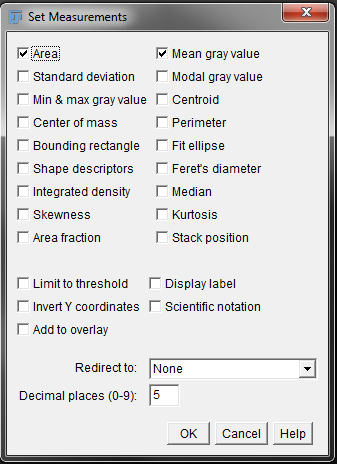
\includegraphics[width=0.4\textwidth]{mod2/figures/set-measurements-dialog.png}
		\caption{Set Measurements Dialog.}\label{fig:set-measurements-dialog}
	\end{center}
\end{figure}

\newpage
\begin{taskbox}{Using the ROI Manager}
Now, we are going to combine ROIs (and the ROI Manager) with measurements -- you will see how powerful this already gets!
\begin{enumerate}
	\item Open the image hela-cells.tif in /mod2/data. Open the ROI Manager and load the previously generated ROI data.
	\item Measure the area and average intensity of the whole cell, the nucleus and the cytoplasm in the green channel and compare the results (Fig. \ref{fig:results-window}).
	
		\begin{minipage}[t]{\linewidth}
		\begin{center}
		\adjustbox{valign=t}{%
			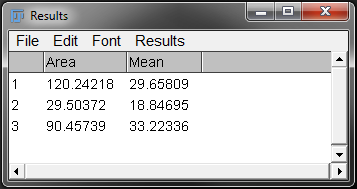
\includegraphics[width=0.3\textwidth]{mod2/figures/results-window.png}%
		}
		\medskip
		\captionof{figure}{Results window showing measurements.}\label{fig:results-window}
		\end{center}
	\end{minipage}
	
	\item Create a ROI in the background of the image (no cell), select the green channel and measure the average intensity again. Name the ROI 'Background' and update the saved ROI file; we will need this for further measurements.
\end{enumerate}	
\end{taskbox}

\section{Changing pixel intensities}
We now have seen various times that an image is represented as a matrix and that we can operate on individual pixels. In this section, we explore basic operations that allow us to modify the values of individual pixels in a ROI or the whole image. As you will see, you have to be careful with these operations, especially when you want to measure and/or compare intensities. However, they can be extremely useful to identify interesting regions of your images or enhance details.

\subsection{Arithmetic}
As an image is a matrix of numbers, we can do usual math on those pixels. We will go through one example where this might be useful and one example to show that things can go wrong if we are not careful.

\begin{taskbox}{Subtracting background levels}
A common task is the subtraction of the background levels of our images to make them comparable (background levels might vary). Subtracting a constant is the most basic background subtraction possible. 

\begin{enumerate}
	\item Open the image hela-cells.tif in /mod2/data. Open the ROI Manager and load the previously generated ROI data that includes the background ROI.
	\item Measure the average intensity in the background and note the value.
	\item Select the overall image \texttt{[Edit > Selection > Select All]} in the green channel. 
	\item Subtract the average background level from the green channel, using \texttt{[Process > Math > Subtract]}. You can also measure the backgrounds of the other color channels and subtract those as well.
\end{enumerate}

\end{taskbox}

\begin{taskbox}{Bit-depth/Format Problems}
A common task is the subtraction of the background levels of our images to make them comparable (background levels might vary). Subtracting a constant is the most basic background subtraction possible. 

\begin{enumerate}
	\item Open the image hela-cells.tif in /mod2/data. Duplicate the green channel.
	\item Look at the histogram of the green channel.
	\item Now, multiply the image by 2.5 - this increases the brightness of the image. 
	\item Generate the histogram again and compare the number of saturated values. As you can see, if the resulting value of a pixel is clipped if we get a value outside our bit-depth. If the result is a real number but our format only allows whole numbers, the resulting value would be rounded. Of course, this was a rather stupid example, but this is a common mistake when you perform more complicated calculations on your images.
	\item if you want, you can convert your image to an appropriate format and compare results.
	\item You can also try to perform the previous invert-example without the conversion to 32-bit.
	\end{enumerate}
	
\end{taskbox}

\subsection{Doing math with two images}
In the previous section, we operated with a single image and constant numeric values. Likewise, we can perform computations that involve two images. Assuming that both images have the same dimensions, we can perform calculations on each pair of pixels at the same position. For example, this type of operation can be used to subtract an image showing only (non-uniform) background from the image showing background + data or we can compare two images by obtaining their difference.

\begin{taskbox}{Background subtraction}
In this example, we are exploring a common method to subtract background information from a time-series. In the given example, we have moving bacteria that were imaged with phase contrast microscopy. The key idea for the background subtraction is that on each pixel, most of the time no bacteria is visible. We therefore create an average image and subtract this image from the original images to increase contrast of moving bacteria.

\begin{enumerate}
	\item Open the image bacteria-tracks.tif in /mod2/data. This image was create from supplementary video 1 of the publication: Rosser et al. (2013) Novel Methods for Analysing Bacterial Tracks Reveal Persistence in Rhodobacter sphaeroides, PLOS Computational Biology, DOI: 10.1371/journal.pcbi.1003276. Please note that this was not the original data, it seems that the supplementary movie was compressed!
	\item Perform a Z-projection to create an average image.
	\item Use \texttt{[Process > Image Calculator...]} to subtract the average image from each image in the original time-series and display the difference in a new window.
	\item Do you see any differences?
\end{enumerate}

Not surprisingly, the authors of the original publication used exactly this approach as the first step in their image processing.

\end{taskbox}

\begin{taskbox}{Math on Masks}
Before, we used the ROI Manager XOR function to obtain the cytoplasm ROI. We can obtain the same result using image masks and image calculations (actually this is likely happening behind the scenes anyway!).

\begin{enumerate}
	\item Open the image hela-cells.tif in /mod2/data. Open the ROI Manager and load the previously generated ROI data that includes the background ROI.
	\item Duplicate just the green channel.
	\item Select the Nucleus ROI and create a mask (look at the previous exercise if you forgot how to proceed). Duplicate the mask.
	\item Now, select the Cell ROI and create another mask.
	\item you should now have two image masks (black-and-white images, see fig. \ref{fig:image-masks}).	
	
		\begin{minipage}[t]{\linewidth}
		\begin{center}
		\adjustbox{valign=t}{%
			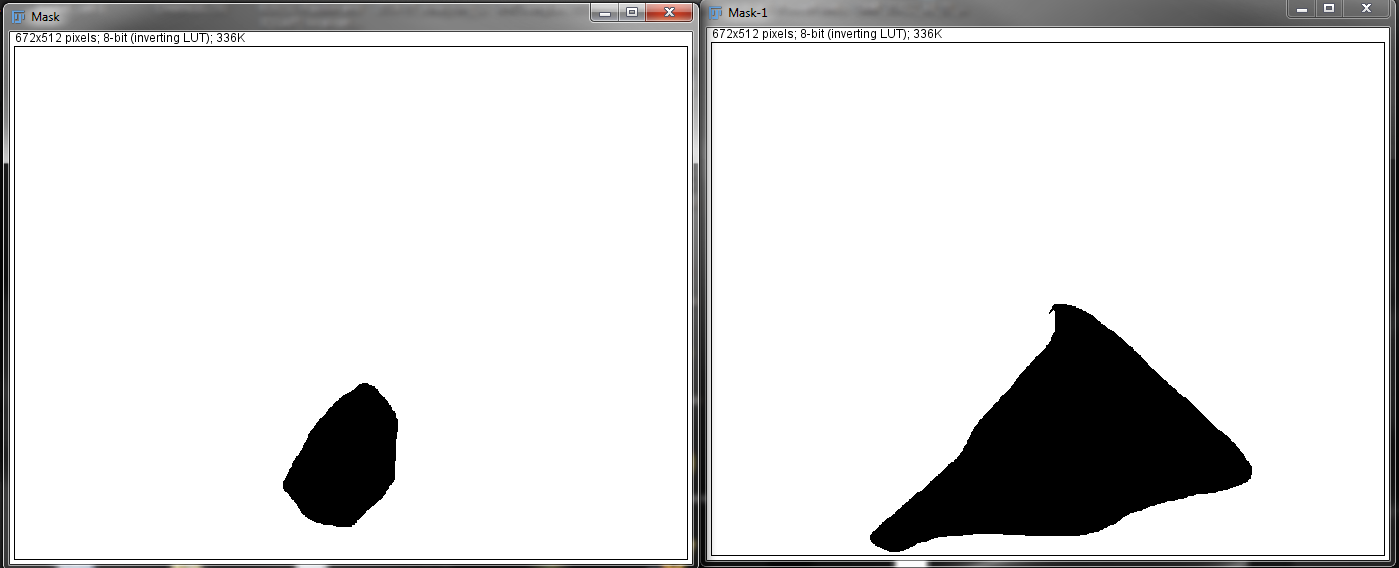
\includegraphics[width=0.8\textwidth]{mod2/figures/image-masks.png}%
		}
		\medskip
		\captionof{figure}{Image Masks.}\label{fig:image-masks}
		\end{center}
	\end{minipage}
	
	\item Calculate the XOR function using the binary data of both images (\texttt{[Process > Image Calculator...]}).
	\item Compare the results with the cytoplasm ROI.
	\item Using \texttt{[Edit > Create Selection]}, you can create a selection from the mask.
\end{enumerate}

\end{taskbox}

\section{Contrast enhancements}
You might already have experience with contrast enhancing of digital images, since most photo-editing software/apps have this function. Low contrast images have small differences in tones and objects are difficult to observe. If the contrast is too high, the tone difference is very high, the picture is 'over-exposed'. Contrast can be adjusted to optimize the appearance of the image. Contrast enhancement primarily changes the LUT, leaving the original data unaffected (it is affected if you apply the changes). Contrast enhancement should be used with care as pixel values are altered and intensity calculations become useless. Therefore, you should avoid contrast enhancements when you analyze intensities (this also applies to the figures that make your point!). Even if you treat all images the same way, you have to make sure that you avoid clipping and that results are not distorted by contrast enhancement.

\begin{taskbox}{Contrast Enhancement and Image Manipulation}
Let's assume you want to show gel data in your manuscript. After performing following steps, can you discuss why contrast enhancement might be considered fraud?
\begin{enumerate}
	\item Open the image gel.tif in mod2/data and duplicate the image (another Fiji sample image).
	\item Adjust Contrast and Brightness and compare images. What is the problem with the contrast-enhanced image (Fig. \ref{fig:contrast-problem})?
	
	\begin{minipage}[t]{\linewidth}
		\begin{center}
		\adjustbox{valign=t}{%
			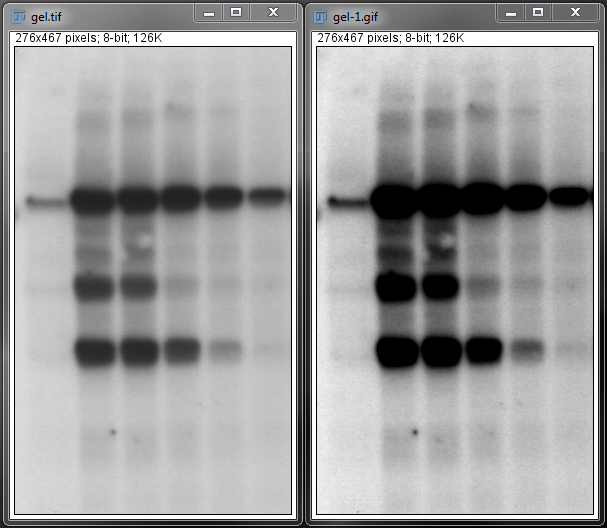
\includegraphics[width=0.8\textwidth]{mod2/figures/contrast-problem.png}%
		}
		\medskip
		\captionof{figure}{Contrast enhancement. The left gel plot shows the original data. Contrast enhancement in the right gel plot shows that you interpretation of this gel might be different.}\label{fig:contrast-problem}
		\end{center}
	\end{minipage}
	
	\end{enumerate}
\end{taskbox}

\subsection{Histogram Normalization}
With normalization, pixel values are normalized according to the minimum and the maximum pixel values in the image and bit-depth. If the minimum pixel value is \emph{pmin} and the maximum is \emph{pmax} in an 8-bit image, then normalization is done as follows:

\begin{equation*}
\mathit{NewPixelValue}=\frac{(\mathit{OriginalPixelValue}-\mathit{pmin})}{(\mathit{pmax}-\mathit{pmin})}\ast
255
\end{equation*}

\begin{taskbox}{Histogram Normalization}

\begin{enumerate}
	\item Open the image hela-cells.tif in /mod2/data and duplicate the green channel. Obtain a histogram.
	\item Use \texttt{[Process > Enhance Contrast]} on the duplicate. Set saturated pixels to 0, tick normalize and not equalize (Fig. \ref{fig:enhance-contrast-dialog}) and obtain a histogram afterwards.
	
	\begin{minipage}[t]{\linewidth}
		\begin{center}
		\adjustbox{valign=t}{%
			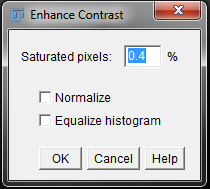
\includegraphics[width=0.3\textwidth]{mod2/figures/enhance-contrast-dialog.png}%
		}
		\medskip
		\captionof{figure}{Enhance Contrast Dialog.}\label{fig:enhance-contrast-dialog}
		\end{center}
	\end{minipage}
	
	\item Compare the histograms. 
	\item Leave the images open; you can also explore different settings.
	
	\end{enumerate}
\end{taskbox}

\subsection{Histogram Equalization}
Equalization converts pixel values so that the values are distributed evenly within the dynamic range. 

\begin{taskbox}{Histogram Equalization}

\begin{enumerate}
	\item Go to the original image showing the green channel.
	\item Use \texttt{[Process > Enhance Contrast]} on the duplicate. Set saturated pixels to 0, tick equalize, not normalize and obtain a histogram.
	\item Compare the histograms. 
	
	\end{enumerate}
\end{taskbox}

\subsection{Local Histogram Equalization}
Histogram equalization could also be performed on a local basis. This becomes powerful, as more local details could be contrast enhanced. In Fiji, you can use local histogram equalization with \texttt{[Process > Enhance Local Contrast (CLAHE)]}.

\section{Colocalization}

